\section{Mass assignment schemes}
For the calculation of a simple cosmological N-body simulation\footnote{Unfortunately, not done in this solution paper}, the particle mesh algorithm is used to calculate the density mesh, which is subsequently used to calculate the gravitational forces in the simulation. This exercise will look at different methods that can be used for the creation of the particle mesh. First the nearest grid point method (NGP) is put under investigation, following with the cloud in cell (CIC) method. Afterwards, an FFT algorithm is build that is able to compute the fourier transform of a given discrete function. The shared code in this question is shown below,

\lstinputlisting[firstline = 289,lastline = 358]{functions.py}

\subsection{Nearest Grid Point (NGP) Method}
The simplest choice for a particle shape is given by,
\begin{equation*}
S(x) = \frac{1}{\triangle x}\delta\left(\frac{x}{\triangle x}\right)
\end{equation*}
For this particle shape the mass assignment scheme is done in the following way. The position of the particle is assigned to be between two cells. This can be done, for example, with the use of the bisection algorithm. Then the differences between the positions of these cells and the position of the particles are taken. If the positional difference between cell 1 and the particle is smaller than the positional difference between cell 2 and the particle, then the complete mass of the particle is assigned to cell 1. The reason that this is called the Nearest Grid Point method is because the total mass of the particle is assigned to it's nearest grid point. To test this algorithm, 1024 particle positions were randomly created (with seed 121) in the ranges $0 \leq x,y,z  \leq 1$. The bisection algorithm is used to get the $x$, $y$, and $z$ positions of the most nearby grid points. Then the differences between the positions of the particles and these most nearby grid points are taken to determine which grid point the mass is assigned to. The mass in this exercise is taken to be fractions of the total mass. So if a cell contains one particle then the mass that it is assigned to is $\frac{1}{1024}$. This is because we want the integral of the density grid to be equal to the total mass of all particles. For this exercise, periodic boundary conditions are used. The code that is used is shown below,

\lstinputlisting[firstline = 18, lastline = 52]{Q5.py}
The output of the code are 4 plots of the $x-y$ grid for $z = 4,9,11,14$, as shown below.

\begin{figure}[h]
\centering
\includegraphics[scale=0.9]{plots/NGD_9.png}
\caption{Mass assignment scheme for $z = 4$ (left figure) and $z = 9$ (right figure).}
\end{figure}
\begin{figure}[h]
\centering
\includegraphics[scale=0.9]{plots/NGD_14.png}
\caption{Mass assignment scheme for $z = 11$ (left figure) and $z = 14$ (right figure).}
\end{figure}
The white spots in the figures are cells which have got no mass assigned to it at all. The dark blue patches seem to be 0 as well but these cells still have a small amount of mass assigned to it. It can be seen from the figures that all figures are equally dense and all four plots also show a quite discrete density mesh. The robustness of this implementation is discussed in the next section.


\subsection{Robustness NGP}

The robustness of the implementation of the NGP can be checked by simply iterating over various $x$ positions between 0 and 16 and check how each cell responds to this position. This check is done for cell 4 and for cell 0. The code used for this robustness check is given below,

\lstinputlisting[firstline = 54, lastline = 75]{Q5.py}

The output of this code is a plot of the fraction of the mass of the particle that is assigned to the cell against the position of the particle.

\begin{figure}[h]
\centering
\includegraphics[scale=0.6]{plots/NGD_test.png}
\caption{The fraction of the mass of the particle assigned to the cell plotted against the position of the particle. The orange line is for cell 0 and the blue line is for cell 4.}
\end{figure}

The figure looks exactly as expected. When the particle enters the cell, all of its mass is assigned to it straight away. As a result the density mess will look very discrete. Also at the boundaries, the mass gets assigned to cell 0 which is due to the circularity. A better method would be to use an interpolation algorithm. Such an algorithm is discussed and tested in the next section.

\subsection{Cloud In Cell (CIC) Method}

The cloud in cell (CIC) method is a mass assignment scheme method that makes use of interpolation. Instead of assigning all the mass of a particle to one grid point, parts of its mass are assigned to multiple grid points. Depending on how far the particle is from the grid point, it will get a fraction of the mass of the particle. In 3D one should image it in the following way. Let a particle have position $(x,y,z)$. The grid points surrounding this particle in 3D can be thought of as a cube. A visualisation is shown in figure \ref{cube}.

\begin{figure}[h]
\centering
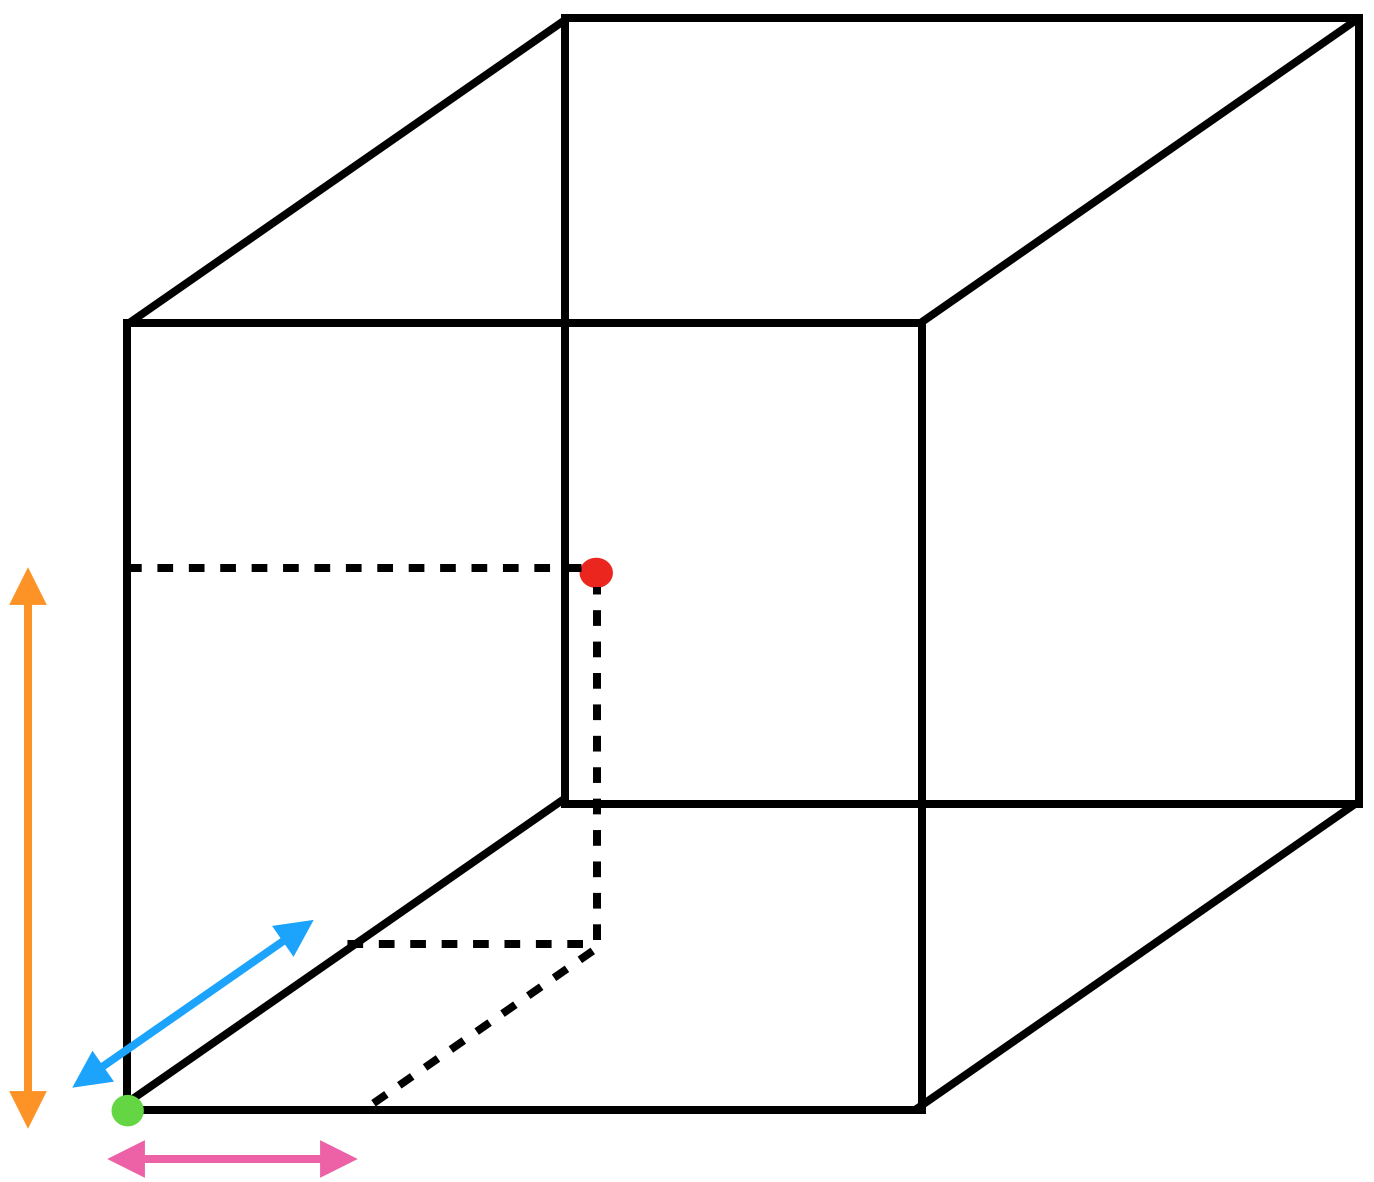
\includegraphics[scale=0.3]{cube}
\caption{Visualisation of a cube surrounding a particle, where the vertices of the cube represent the grid points of the density mesh.}
\label{cube}
\end{figure}
The particle in this figure is deliberately not placed at the center of the cube to show that each grid point (vertice) gets a different amount of fraction of the mass of the particle. The green grid point is second closest to the particle (the closest is the grid point just above this one). Using interpolation, the mass it gets assigned to is now the size of the pink arrow times the size of the blue arrow times the size of the orange arrow. Using this logic, it can be seen that the grid point opposite the green one (which is furthest away from the particle) gets less mass of the particle. So to summarize, the mass of the particle is split up in 8 bits. Each bit is determined by how close the particle is to the grid point. The code that is used to create this algorithm, including the robustness check, is shown below,

\lstinputlisting[firstline = 77, lastline = 163]{Q5.py}

The output of the code are again 4 plots of the $x - y$ grid for $z = 4,9,11,14$, together with the same robustness check plot as shown in the previous section.

\begin{figure}[h]
\centering
\includegraphics[scale=0.9]{plots/CIC_9.png}
\caption{Mass assignment scheme for $z = 4$ (left figure) and $z = 9$ (right figure).}
\label{cic1}
\end{figure}

\begin{figure}[h]
\centering
\includegraphics[scale=0.9]{plots/CIC_14.png}
\caption{Mass assignment scheme for $z = 11$ (left figure) and $z = 14$ (right figure).}
\label{cic2}
\end{figure}

\begin{figure}[h]
\centering
\includegraphics[scale=0.6]{plots/CIC_test.png}
\caption{The fraction of the mass of the particle assigned to the cell plotted against the position of the particles. The orange line is for cell 0 and the blue line if for cell 4.}
\label{cic_test}
\end{figure}

The white spots represent again cells which do not have mass assigned to it at all. The amount of white patches is, however, less in these 4 figures than the amount of white patches in the 4 figures shown in section 5.1. In addition, the patches that show mass seem to overflow a tiny bit from one to another (i.e. there seems to be some smoothness in the figures). Looking at figure \ref{cic_test}, one can see that this method is less discrete than the NGP method. The amount of mass assigned to the cells one and four increases as it approaches the grid point and decreases again when it moves away from the grid point. Just as expected what should happen when using interpolation.
\clearpage

\subsection{Fast Fourier Transform}

A method for computing the fourier transform numerically is the fast fourier transform. To be more specific, the method that is going to be discussed in this section is the Cooley-Tukey FFT. The fast fourier transform makes use of the fact that the fourier transform is symmetric. The discrete fourier transform is given by,

\begin{equation*}
X_k = \sum_{n=0}^{N-1}x_n e^{-\frac{2\pi i}{N}nk}
\end{equation*}
where $k$ is an integer that is ranging from 0 to $N-1$. Here $N$ is the number of data points. The simplest Cooley-Tukey algorithm splits the function $x_n$ into two parts. It is split into a sum over the even indices, and a sum over the odd indices,
\begin{equation*}
X_k = \sum_{m=0}^{\frac{N}{2} - 1} x_{2m}e^{-\frac{2\pi i}{N}(2m)k} + \sum_{m=0}^{\frac{N}{2}-1}x_{2m+1}e^{-\frac{2\pi i}{N}(2m+1)k}
\end{equation*}
In the second sum, it is possible to factor the term $e^{-\frac{2\pi i}{N}k}$ out. So now we get,
\begin{equation*}
X_k = \sum_{m=0}^{\frac{N}{2}-1}x_{2m}e^{-\frac{2\pi i}{N/2}mk} + e^{-\frac{2\pi i}{N}k}\sum_{m=0}^{\frac{N}{2}-1}x_{2m+1}e^{-\frac{2\pi i}{N/2}mk}
\end{equation*}
Now due to symmetry we have that $X_{k + \frac{N}{2}}$ can also be obtained with the odd and even parts of $x_n$,
\begin{gather*}
X_{k+\frac{N}{2}} = \sum_{m=0}^{\frac{N}{2}-1}x_{2m}e^{\frac{-2\pi i}{N/2}m(k+\frac{N}{2})} + \sum_{m=0}^{\frac{N}{2}-1} x_{2m+1}e^{-\frac{2\pi i}{N}(2m+1)(k+\frac{N}{2})}\\
=  \sum_{m=0}^{\frac{N}{2}-1}x_{2m}e^{\frac{-2\pi i}{N/2}m(k+\frac{N}{2})}\cdot e^{-2\pi m i} + e^{-\frac{2\pi i}{N}(k + \frac{N}{2})}\sum_{m=0}^{\frac{N}{2}-1} x_{2m+1} e^{-\frac{2\pi i}{N/2}m(k+\frac{N}{2})}\\
= \sum_{m=0}^{\frac{N}{2}-1}x_{2m}e^{\frac{-2\pi i}{N/2}m(k+\frac{N}{2})}\cdot e^{-2\pi m i} + e^{\frac{2\pi i}{N}k}e^{-\pi i}\sum_{m=0}^{\frac{N}{2}-1} x_{2m+1} e^{-\frac{2\pi i}{N/2}m(k+\frac{N}{2})}
\end{gather*}
The terms $e^{2\pi m i}$ and $e^{\pi i}$ are 1 and minus 1 respectively, and therefore the equation above becomes,
\begin{equation*}
X_{k+\frac{N}{2}} =  \sum_{m=0}^{\frac{N}{2}-1}x_{2m}e^{\frac{-2\pi i}{N/2}m(k+\frac{N}{2})} - e^{\frac{2\pi i}{N}k}\sum_{m=0}^{\frac{N}{2}-1} x_{2m+1} e^{-\frac{2\pi i}{N/2}m(k+\frac{N}{2})}
\end{equation*}
Using this symmetry makes computing the fourier transform much more efficient. Using these equations recursively makes this fast fourier transform extremely efficient. There is, however, another way to compute it with the use of bit-reversal. This is known as another variant of the Cooley-Tukey algorithm but is not used in this solution paper. The code that has been used to compute this is shown below,

\lstinputlisting[firstline = 165, lastline = 216]{Q5.py}
The output of this code is the fourier transform of the function $\cos(40\pi x)$ gotten from the own implementation, the one from scipy and the analytical solution.

\begin{figure}[h]
\centering
\includegraphics[scale=0.6]{plots/FFT_1D.png}
\caption{The fourier transform of $\cos(40\pi x)$, where the blue dotted line is the solution from scipy, the orange line is the own implementation and the red lines is the analytical solution}
\label{FFT_1D}
\end{figure}

It can be seen from the figure \ref{FFT_1D} that the scipy solution and the own implementation are exactly the same. The analytical solution is obtained by noticing that the fourier transform of this particular function is simply a delta function,

\begin{equation*}
\mathrm{FT} \propto \delta\left(\omega - 40\pi\right) + \delta\left(\omega + 40\pi\right) 
\end{equation*}
where $\omega$ are the frequencies. This delta function is of course analytically simply a vertical line. However, because we have a discrete function, it is not possible to create a vertical line that goes to infinity, and therefore a small dispersion will be seen in the graph. The positions of the peaks are at the exact same spot, which is as expected. Note that there are two peaks, this is because in fourier space we have negative and positive frequencies.

\subsection{Fast Fourier Transform in 2D and 3D}

Now that we've shown that the 1D fourier transform seems to work fine, it is also possible to do this in 2 and 3 dimensions. This can be done by simply fourier transforming over each dimension. So for the 2D FFT this would be transforming the rows and columns separately, and for the 3D FFT this would be transforming the arrays in the x, y, and z axis separately. The code that is used for this is shown below,

\lstinputlisting[firstline = 218, lastline = 354]{Q5.py}
The output of the code is for the 2D fft the fourier transform of the function $\cos(0.2\pi(X+Y))$, where $X$ and $Y$ are 2D matrices, with the use of the own implementation and the one from scipy. I did not manage to convert the axes of this 2D plot to the right frequencies, and therefore I also did not manage to plot the analytical version. The analytical version would resemble a delta function again, but now in 2D. It would peak at $\omega_x = \omega_y = 0.2\pi$ and $\omega_x = \omega_y = -0.2\pi$. For the 3D plot, the multivariate gaussian has been fourier transformed, using the own implementation and the own from scipy. This 3D matrix has been sliced to get the x-y, y-z, and x-z grids at the center of the matrix.
\begin{figure}[h]
\centering
\includegraphics[scale=0.5]{plots/real_space_2D.png}
\caption{The real-spaced function $\cos(0.2\pi(X+Y))$.}
\end{figure}
\begin{figure}[h]
\centering
\includegraphics[scale=0.8]{plots/FFT_2D.png}
\caption{The fourier transform of the 2D function. Left: scipy fourier transform, right: own implementation}
\end{figure}
\begin{figure}[h]
\centering
\includegraphics[scale=0.85]{plots/gauss_XY.png}
\caption{The fourier transform of the 3D function. Left: scipy fourier transform, right: own implementation. This figure represents the $x-y$ grid.}
\end{figure}
\begin{figure}[h]
\centering
\includegraphics[scale=0.85]{plots/gauss_YZ.png}
\caption{The fourier transform of the 3D function. Left: scipy fourier transform, right: own implementation. This figure represents the $y-z$ grid.}
\end{figure}
\begin{figure}[h]
\centering
\includegraphics[scale=0.85]{plots/gauss_XZ.png}
\caption{The fourier transform of the 3D function. Left: scipy fourier transform, right: own implementation. This figure represents the $x-z$ grid.}
\end{figure}

Both the figures of the 2D fourier transform and the 3D fourier transform seem to match the scipy implementation quite well. The 2D fourier transform should have been two scatter points without any dispersion. However, as mentioned in the previous section, numerically this can not be computed since the delta function is not defined numerically. We can see also that the amplitudes of these yellow dots are extremely high which indicates that this delta function is done relatively well. We'd expect these amplitudes to go to infinity but, of course, this is numerically not possible. The analytical solution would match this one quite well, though it would not have these dispersion lines seen in the x and y directions. 
\clearpage